% !TeX root = thesis_guide.tex
% chktex-file 1 chktex-file 21 chktex-file 46

%==============================================================================
\chapter{Tips and tricks}%
\label{sec:tips}\index{tips}
%==============================================================================

\LaTeX{} file: \url{./guide_tips.tex}\\[1ex]
\noindent
Over time I have collected quite a lengthy list of things you should
\enquote{Do} and \enquote{Not Do} (at least in my head) that I think
it is useful to write down early in the document, so that you may
actually read them!  In this chapter I first tell you how to get
and use the style file and then give some tips.
I have also started to add a list of common English mistakes,
especially those made by German speakers!

%------------------------------------------------------------------------------
\section{How to use the \Package{ubonn-thesis} style}%
\label{sec:tips:howto}
%------------------------------------------------------------------------------

My original idea with this document was that you also look at the \LaTeX{} that
is used to create it, in order to find out how things are done.
I have therefore usually not usually given the \LaTeX{} commands in the printed
document, but assumed that you would have a look at the \LaTeX{} source.
To help you with this, each chapter contains a link to the relevant
file at the top. This link should work if you have compiled the guide
yourself and are in the \texttt{guide} subdirectory of the
\texttt{ubonn-thesis} directory tree.
As of version 7.0 of the guide,
I have started using the \Package{showexpl} package that allows me to show
both the \LaTeX{} and the result automatically.
Hence in some places you will find compiled \LaTeX{} and the source code side by side.
The files that make up this document are available in a Git repository and as a \texttt{tar} file.
To get the latest Git version give the command:

\begin{bashlisting}
git clone https://bitbucket.team.uni-bonn.de/scm/uni/ubonn-thesis.git
\end{bashlisting}
\noindent
If you want to checkout a particular version you can give the command:
\begin{bashlisting}
git clone --branch vN.M \
  https://bitbucket.team.uni-bonn.de/scm/uni/ubonn-thesis.git
\end{bashlisting}
Note that you have to be in the University of Bonn network for the clone commands to work.
\noindent
The tar file (and the tag tree (as of version 1.5)) also includes
the guide as a PDF file: \texttt{thesis\_guide.pdf}.  It can be
obtained from:\\
\url{http://www.pi.uni-bonn.de/teaching/uni-bonn-thesis}
and\\
\url{http://www.pi.uni-bonn.de/lehre/uni-bonn-thesis}.

\par\noindent
Once you have the files, you can then give the command:
\begin{bashlisting}
make new [THESIS=dirname] [TEXLIVE=YYYY]
\end{bashlisting}
to create a new directory with several files to help you get
started. By default the directory name will be \texttt{mythesis}.
If you want to write a thesis that uses the astronomy style of references
(\Option{authoryear} style and a bibliography at the end of each chapter)
give the command \enquote{\texttt{make astro [THESIS=dirname]}}.
% If you choose a different name, you have to adjust the \Macro{include}
% commands inside \texttt{./dirname.tex}.
To compile\index{compiling} your thesis switch to your new directory
\verb+cd mythesis [or dirname]+ and try:
\begin{bashlisting}
make thesis
\end{bashlisting}
See \cref{sec:tips:options} for a list of the options that can be passed to the package.
I no longer support versions of \TeXLive older than 2011,
and can only test things for \TeXLive 2014 and later.
% you should really update to a newer version!
% If this is not possible, use the command \enquote{\texttt{make new09}}
% followed by \enquote{\texttt{make thesis09}}
% or \enquote{\texttt{make thesis BIBTEX=bibtex}}.

As of version 6.0, \Command{make thesis} uses the \Command{latexmk}\index{latexmk} command for compilation.
\Command{latexmk} looks at your logfile and decides how many times \Command{pdflatex} etc.
have to be run.
If you use \Package{feynmf} or \Package{feynmp} you should use the commented out version
of the \Command{LATEXMK} variable that includes the \Option{-shell-escape} option.\footnote{%
  I got this information from \url{https://tex.stackexchange.com/questions/374160/how-to-have-latexmk-always-use-shell-escape}.}
For details on how to compile a glossary with \Command{latexmk} see \cref{sec:app:glossary}.
If for some reason \Command{latexmk}\index{latexmk} does not work you can use the command
\Command{make thesis11} instead.
The tool \Command{pplatex}\footnote{%
Can be downloaded from \url{https://github.com/stefanhepp/pplatex}.
}
is supposed to provide a nicely formatted version of the \LaTeX\ output on the command line.

My original idea was that the style file should work for all recent
\TeX\ installations.  However, some of the packages I recommend have
been changing quite a lot over the past few years.
You should therefore set the \TeXLive version you are using appropriately.
The default setting is 2016.\footnote{%
Setting the \TeXLive version to one that is lower than your installation should not cause any problems.}
This is also the setting to use for an up-to-date version of MikTeX (2.9).
Things should compile without any changes if you use \TeXLive 2016 or later.
Look in the style file to see what changes are made depending on the year you use.
You can change the \TeXLive version when you make a new thesis
by giving a command like \enquote{\texttt{make new TEXLIVE=2013}}. %\footnote{%
% For even older versions of \TeXLive use the command \enquote{\texttt{make new09}}.
% This turns off the use of \Package{biblatex}.}
If you switch \TeXLive versions do a
\enquote{\texttt{make clean cleanbbl cleanblx}} in between.

Note that as of version 2.1, the main file for the thesis
(\texttt{mythesis.tex}), the \texttt{Makefile} and the style file
(\texttt{ubonn-thesis.sty}) are copied into your \texttt{mythesis}
subdirectory. This means that if you update the \Package{ubonn-thesis}
you can look for differences between the new style file and the one
you have. It also implies that if you want the update to have an
effect on your thesis you should copy the \texttt{Makefile} and
\texttt{ubonn-thesis.sty} into the directory with your thesis.
For more details see \cref{sec:tips:update}.

As of version~4.0 of the package, you specify the type of thesis and the stage as options
to the \Macro{documentclass} or to the \Package{ubonn-thesis} package.
These options select the appropriate title and cover pages.
The following thesis types exist:
\begin{description}\setlength{\parskip}{0pt}\setlength{\itemsep}{0pt}
\item[PhD] a PhD thesis;\index{PhD}\index{thesis!PhD}
\item[Master] a Master thesis;\index{MSc}\index{thesis!Master}
\item[Diplom] a Diplom thesis;\index{Diplom}\index{thesis!Diplom}
\item[Bachelor] a Bachelor thesis.\index{BSc}\index{thesis!Bachelor}
\end{description}
The following stages exist:
\begin{description}\setlength{\parskip}{0pt}\setlength{\itemsep}{0pt}
\item[Draft] you are still writing your thesis;
\item[Submit] you are ready to submit your thesis;
\item[Final] the final version of your thesis.
  For PhD theses this is the version that goes to ULB\@;
\item[PILibrary] final version of your thesis with an extra cover page\index{cover}
  including an abstract for the PI library.
\end{description}
%
%\noindent
%In the main thesis file, \texttt{mythesis.tex}, you need to specify
%which cover page should be used:\index{cover page}
%\begin{description}
%\item[\texttt{PhD\_Submit\_Title.tex} and \texttt{PhD\_Final\_Title.tex}:]
%  the title pages for a PhD thesis;\index{PhD}\index{thesis!PhD}
%\item[\texttt{Master\_Submit\_Title.tex} and \texttt{Master\_Final\_Title.tex}:]
%  the title pages for an MSc thesis;\index{MSc}\index{thesis!Master}
%\item[\texttt{Diplom\_Submit\_Title.tex} and \texttt{Diplom\_Final\_Title.tex}:]
%  the title pages for a Diplom thesis;\index{Diplom}\index{thesis!Diplom}
%\item[\texttt{Bachelor\_Title.tex}:]
%  the title pages for a BSc thesis.\index{BSc}\index{thesis!Bachelor}
%\end{description}
%For the printed version for the department library you also need to
%include the appropriate cover page (with an abstract):\index{cover}
%\begin{description}
%\item[\texttt{PhD\_Cover.tex}:]
%  The cover page for a PhD thesis;
%\item[\texttt{Diplom\_Cover.tex}:]
%  The cover page for a Diplom thesis;
%\item[\texttt{Master\_Cover.tex}:]
%  The cover page for an MSc thesis.
%\end{description}
%This extra cover should not be included for the version of the PhD
%thesis that is submitted to the university library (ULB).
See \cref{sec:submit} for some more details about thesis submission.

If you change the stage of your thesis from say \Option{Draft}\index{Draft} to \Option{Submit}\index{Submit}
you may encounter \Package{biblatex} errors.
These can be fixed by giving the command \texttt{make cleanall; make}.

If you are not a member of the
\foreignquote{ngerman}{Physikalisches Institut} you should
also change \Macro{InstituteName}, \Macro{inInstitute} and
\Macro{InstituteAddress}. The style file \texttt{ubonn-thesis.sty}
already contains the appropriate definitions for PI, HISKP, IAP and
AIfA.

All packages that are needed should be part of your \TeX\
installation. If not you may have to install them or ask your system
administrator to do so.

If you just want to make the cover pages, use the file
\texttt{cover\_only.tex}.  Be sure to adapt the font selected in
\texttt{ubonn-thesis.sty} to the font you actually used in your
thesis. Be aware that not all font sizes are available in all font
collections. If you used the default \LaTeX{} font in your thesis,
then choose \Package{lmodern}\index{font!lmodern} in the style file.

The main file for this guide is \texttt{guide/thesis\_guide.tex} and
it includes the \LaTeX{} files in the directory \texttt{./guide} and
some of the Feynman graphs in the directories 
\texttt{./feynmf}, \texttt{pyfeyn}, \texttt{pyfeynhand} and \texttt{./tikz}.
Again this guide should compile without changes for
\TeXLive 2016 or later. For earlier versions set \Macro{texlive} in
\texttt{thesis\_guide.tex} to the appropriate value.
Set the default font to \Package{txfonts} for \TeXLive 2011.
% If you want to compile the guide with \TeXLive older than 2011,
% it is probably easier to switch from \Package{biblatex} to traditional \BibTeX.
% This is done via the \texttt{make new09} command.

%The guide will not compile for \TeXLive versions lower than 2012,
%as the \Package{subcaption} package and the way to load it was different earlier.


%------------------------------------------------------------------------------
\section{Options that can be passed to \Option{ubonn-thesis}}%
\label{sec:tips:options}\index{options}
%------------------------------------------------------------------------------

From version~3.0 onwards it is possible to change things
in the style file by passing options to it.
A few default packages also changed with this version.
\Package{subfig} \(\to\) \Package{subcaption} and
\Package{longtable} \(\to\) \Package{xtab}.
The syntax \Option{siunitx} and \Option{siunitx=true} is equivalent.
Use \Option{siunitx=false} to turn off an option.
The following options exist:\\

\tablehead{Option & Default & Description \\
  \midrule}
\tablelasttail{\bottomrule\\}
\xentrystretch{-0.05}
\begin{xtabular}{llp{10.0cm}}
  PhD & false & A PhD thesis.\\
  Master & false & A Master thesis.\\
  Diplom & false & A Diplom thesis.\\
  Bachelor & false & A Bachelor thesis.\\
  Draft & true & Draft version of the thesis.\\
  Submit & false & Version of the thesis to be submitted.\\
  Final & false & Final version of the thesis (for PhD theses ready to go to ULB).\\
  PILibrary & false & Final version including an extra cover page for the PI library.\\
  thesistype & Unknown & Specify the thesis type.\\
  thesisversion & Draft & Specify the stage of the thesis.\\
  texlive & 2016 & Specify the \TeXLive version.
    You can also use the older command \verb|\newcommand*{\texlive}{2016}|.\\
  newtx & true & Use the \Package{newtx} font packages (newer version of \Package{txfonts}).\\
  txfonts & false & Use a Times-Roman-like font.\\
  palatino & false & Use a combination of Palatino, Courier and Helvetica fonts.\\
  subcaption & true & A package for making sub-figures (and sub-tables) and captions for them.\\
  subfig & false & A package for making sub-figures and captions for them.\\
  subfigure & false & A package for making sub-figures and captions for them (deprecated).\\
  xtab & true & A package for tables that are longer than one page.\\
  longtable & false &  Another package for tables that are longer than one page.\\
  supertabular & false &  Another package for tables that are longer than one page.\\
  biblatex & true & Include \Package{biblatex}.\\
  siunitx & true & Use the \Package{siunitx} package for typesetting units.\\
  eVkern & false & Apply a kern of -0.1em to \si{\eV} in order to move \enquote{e} and \enquote{V} closer together.
  This is not necessary if you use the \Package{newtx} font package.\\
  dcolumn & true & A package for helping to align things in tables.\\
  physics & false & Useful mathematical constructions for physics.\\
  hepparticles & true & Standardised names and formatting for particle physics.
    This loads \Package{hepnicenames} and \Package{heppennames}.\\
  hepitalic & true & Use italics rather than upright letters for particles.\\
  mhchem & true & A nice package for chemical elements and processes.\\
  bookmark & true & use \Package{bookmark} package to improve bookmarks in PDF file.\\
  feynmf & false & Include the \Package{feynmf} package for Feynman graphs.\\
  feynmp & false & Include the \Package{feynmp} package for Feynman graphs.\\
  titlesec & false & Use the \Package{titlesec} package for formatting chapter titles.\\
  astrobib & false & Adjust \Package{biblatex} options to conform to the usual astronomy style.\\
  floatopt & true & Adjust settings that control the number and placement of floats.\\
  todonotes & false & Turn on use of the \Package{todonotes} package and define \Macro{mynote}.\\
  shownotes & false & Show the ToDo notes (also turns on \Option{todonotes}).\\
  cleveref & false & Turn on use of the \Package{cleveref} package.\\
  clevercaps & true & Capitalise Fig., Table etc.\\
  firstinits & false & Use \Option{firstinits} instead of \Option{giveninits} for \Package{biblatex}.\\
  backref & true & The bibliography lists where the reference is cited.
    This option is very useful when writing your thesis,
    but should probably be turned off for the final version.\\
  backend & biber & Specify the backend to use for \Package{biblatex}.
    Possibilities are \Option{biber}, \Option{bibtex} or \Option{bibtex8}.\\
  bibencoding & & Set the encoding for the bibliography (usually not needed).\\
  bibstyle & numeric-comp & Specify the style to use for the references.
    Standard values are \Option{numeric-comp} or \Option{alphabetic}.\\
\end{xtabular}

Some default option values are adjusted depending on the \TeXLive version.
See the \texttt{ubonn-thesis} style file to find out what is changed.

If you use \LuaLaTeX or \XeLaTeX,
the \Option{newtx} and \Option{txfonts} options select the TeX Gyre Termes font,
while the \Option{palatino} option selects the TeX Gyre Pagella font.
Depending on the font you use, you may find that the \enquote{e} and \enquote{V} in \si{\eV}, \si{\MeV} etc.\
are too far apart.
You can pass the option \Option{eVkern} to \Package{ubonn-thesis} in order to move them 0.1em closer together.\footnote{%
This option has no effect for \TeX\ Live 2011 and older, as \Package{siunitx}
adjusted the spacing internally using the parameter \Option{eVcorra}.
It is not needed if you use the \Package{newtx} font package.}


%------------------------------------------------------------------------------
\section{Do}%
\label{sec:tips:do}
%------------------------------------------------------------------------------

\begin{itemize}
\item Have 1--2 other people read your thesis well before you are
  supposed to submit it. Do not ask too many; everyone has their own
  opinions on how things should be written, how much detail should be
  included etc.\ and these opinions will not necessarily agree with
  each other!

\item Write \enquote{nice} \LaTeX. It makes it much easier to find mistakes
  in your document. If you like to use the keyboard rather than the
  mouse when moving round in a document, turn on \enquote{auto-fill-mode
  (emacs)}\index{emacs} or its equivalent in any other editor, so
  that line breaks are inserted.

\item Make sure every table and figure is referenced in the text. I
  get very irritated when I suddenly find a figure that is not
  described in the text. A useful package to check this is
  \Package{refcheck}.\footnote{%
  There is a conflict if you use \Package{refcheck}, \Package{subcaption} and \Package{hyperref} together.
  See \url{http://tex.stackexchange.com/questions/273970/conflict-refcheck-subcaption-packages-for-label-with-underscores} for a workaround.}
  You need to run \LaTeX\ one more time for it to
  work. It indicates both in the log file and the resulting PDF which
  figures, tables, equations and sections are referenced.

\item Use a units package to format numbers and their units. Recent
  versions of \LaTeX\ include the \PackageG{siunitx} package, which
  is a superior replacement of \Package{SIunits}. I used to
  use \Package{SIunits}, or rather \Package{hepunits} which is
  built on top of \Package{SIunits}, and defines common particle
  physics units such as \si{\GeV}. Use of these packages is
  discussed in \cref{sec:tips:units}.
  An alternative is the \Package{units} package.

\item Define any complicated symbols once you use them more than
  once:
\begin{tcblisting}{listing only}
\newcommand*{\etajet}{\ensuremath{\eta_{\text{jet}}}\xspace}
\end{tcblisting}
  If you decide at a later date that jet should be a superscript
  rather than a subscript you only have to change this in one place!

  Note that Kopka~\cite{kopka04}
  recommends using \Macro{newcommand*} rather than \Macro{newcommand}
  for short commands.

\item If you use normal words in superscripts or subscripts (or
  anything else in math mode) enclose them in \Macro{text}. You can
  also use \Macro{mathrm} or \Macro{textrm}. However, if you then use
  the same symbols in slides with a sans-serif font, the text may well
  continue to be in a
  serif font.\\
  {\sffamily Compare: A common jet energy cut at the LHC is now
    \(p_{T}^{\text{jet}} > \SI{20}{\GeV}\), while at HERA we typically
    used \(p_{T}^{\mathrm{jet}} > \SI[detect-family=false]{6}{\GeV}\).
    % \ifthenelse {\texlive < 2011} {%
    %   used \(p_{T}^{\mathrm{jet}} > \SI[obeyfamily=false]{6}{\GeV}\).
    % }{%
    %   used \(p_{T}^{\mathrm{jet}} > \SI[detect-family=false]{6}{\GeV}\).
    % }
  }
  The \si{\GeV} in the first expression is in sans-serif. This is
  because the
  \Macro{sisetup}\texttt{\{detect-family=true\}} % \footnote{\Option{obeyall} in \TeXLive 2009.}
  option is set in \texttt{ubonn-thesis.sty}
  (see \cref{sec:tips:siunitx}).  I used the option
  \Option{detect-family=false} % \footnote{\Option{obeyfamily=false} in \TeXLive 2009.}
  for the \Macro{SI} command in the 2nd expression.
  In the first expression I use \Macro{text} for \enquote{jet}, while
  I use \Macro{mathrm} in the second expression.

\item Use \Macro{xspace} and
  \Macro{ensuremath} in all commands where you would
  like to use a symbol both in text mode and in math mode. Without
  \Macro{xspace} you have to make sure that you end every symbol with
  \texttt{\textbackslash} or \texttt{\{\}}, otherwise the space is used
  to signify the end of the symbol, e.g.\ in \LaTeX we have to pay
  attention otherwise the symbol and the next word run together.

\item Decide how you want to write abbreviations for particles and
  stick to it --- you should probably define the particle names in your
  style file and always use them (also for quarks).
  There are packages \Package{hepnicenames} and \Package{heppennames},
  which use \Package{hepparticles}.\footnote{%
    Note that \Package{hepnicenames} automatically includes \Package{heppennames},
    so it is sufficient to include \Package{hepnicenames} to be able to use both sets of definitions.}
  These packages have many predefined particles and a standard convention for naming.
  It is easy to add further definitions.
  See \cref{sec:tips:hepparticles} for some more details on how to write particles
  that are relevant for particle physics.

\item Decide how you want to write coordinate axes\index{coordinates}
  and stick to it. Far too often I see text like: \enquote{The proton
    beam defines the Z direction, while the interaction point is
    denoted as \((x_{0}, y_{0}, z_{0})\). The polar angle is measured
    with respect to the z axis and \(\cot\theta = p_{Z}/\pT\)}. Which is
  the best way of writing the coordinates? As \(x\), \(y\) and \(z\) are
  often used for kinematic variables, there are arguments in favour of
  \((X, Y, Z)\).

\item Use \Macro{enquote} from the \PackageG{csquotes} package to
  quote text rather than using explicit quotation marks. This has the
  advantage that consistent quotation marks are used everywhere (also
  if they are nested) and that they are also correct for the language
  (and dialect\footnote{%
    By default, British (UK) English\index{British English}\index{UK English}
    uses `British quoted text' for outer quotation marks,
    while American (US) English\index{American English}\index{US English}
    uses \foreignquote{USenglish}{American quoted text}. In this guide
    (and in \texttt{ubonn-thesis.sty})
    \foreignquote{USenglish}{American (US) quotes} are used even if you
    write in British (UK) English.})
  you are writing your thesis in.
  You can also see in \cref{sec:intro} how this works, even
  when switching languages inside a paragraph.

\item Use sizes that depend on the font size, \texttt{em}\index{em}
  (width of \enquote{M}) and \texttt{ex}\index{ex} (height of \enquote{x}), for
  spacing that should change with the text size. Use absolute sizes
  \texttt{cm, mm, pt} etc.\ where they are appropriate, e.g.\ title
  pages, boxes, etc. \Macro{quad} and
  \Macro{qquad} are also useful sizes in tables and
  equations.

\item Add a \textbackslash{} (or \{\}) after abbreviations that end with a full
  stop such as e.g.\ if followed directly by text. If you do not, an
  end of sentence space is added rather than a normal interword
  space. Note that \textbackslash{} is not needed (but does no harm)
  after abbreviations that only consist of capital letters:\\
  compare \enquote{e.g. my name is Ian C. Brock} % chktex 12
  and \enquote{e.g.\ my name is Ian C.\ Brock},
  where \textbackslash{} was included in the second version. In this
  example the difference is small. However, if \LaTeX{} increases the
  spacing between words to fill a line the effect is more obvious.

\item If a capital letter ends a sentence you should add the
  command \Macro{@} before the full stop, e.g.\
  \verb|\ldots as discussed in the chapter on QCD\@.|
  which produces \ldots as discussed in the chapter on QCD\@.
  This is necessary, as otherwise only an interword space is used
  before the next sentence.

\item Ask someone (me) if you cannot easily find out how to solve
  formatting problems. I once saw a thesis in German, where the
  author wanted to use commas instead of full stops in numbers and
  wrote numbers as \verb+\(2,\!47\)+ to produce \(2,\!47\) instead of
  \(2,47\). There are usually much better solutions, e.g.\
  \verb+\num{2.47}+ with the \Package{siunitx} package produces
  \num{2.47} in English and \foreignlanguage{ngerman}{\num{2.47}} in
  German. In the end such solutions will save you time!

\item Use punctuation in equations and \enquote{\dif}, i.e.\ \Macro{dif} for
  derivatives,\index{derivative} e.g.
  \begin{equation*}
    \int y\,\dif x.
  \end{equation*}
  This is also one of the the very few places, where it makes sense
  to put some spacing in by hand --- normally you should leave this to \TeX.
  Note that the \Package{physics} package provides the command \verb|\dd{x}|,
  which does the spacing for you.
\begin{tcblisting}{listing side text}
\begin{equation*}
  \int y \dd{x}\,.
\end{equation*}      
\end{tcblisting}

\item Pay attention to the alignment of numbers in
  tables. \Package{siunitx} provides the \Option{S} column specifier to
  help with this. Packages such as \Package{dcolumn} also provide assistance.
\end{itemize}

Not really a strict \enquote{Do}: I highly recommend that you use an
integrated environment for editing and compiling your thesis.
If you are use macOS or Windows you probably get TeXShop or TeXworks by default.
\TeXstudio is based on \TeXmaker and is available for Linux,
Windows and macOS\@.
It used to be my preferred \LaTeX\ environment under all systems!
In the past couple of years,
I have switched to the Visual Studio Code\index{Visual Studio Code} editor instead.
The main reason for this is so that I can use the same program
for editing scripts, e.g.\ a \File{Makefile} as I use for \LaTeX\ code.
The \textsf{LaTeX Workshop}\index{LaTeX Workshop@\LaTeX\ Workshop} extension is being actively developed
and is very nice.
The \Package{Spell Right} spelling checker works very well
and I have also activated the use of \Package{ChkTeX} to improve my \LaTeX\ syntax.
Under Linux you can also use Kile\index{kile} or the way I used to work
was to use \texttt{emacs}\index{emacs} and AUCTeX.
Note that the RefTeX\index{RefTeX} mode in \texttt{emacs} also provides powerful
tools for finding cross-references and the names of citations easily.

One advantage of such environments is that it is usually
possible to switch between a position in your output file
and the relevant place in the source code and vice versa.
This makes it much quicker to fix
things when you spot an error in your output PDF file. You can usually
also step through the errors when you try to compile your file and fix
them directly. In addition, they know which environments and
mathematical symbols exist, which can speed things up if you have not
been working with \LaTeX\ for the past 20 years!

More details on integrated environments and installing \TeX\ for different systems can be found
in \cref{sec:app:tex}.


%------------------------------------------------------------------------------
\section{Do not}%
\label{sec:tips:dont}
%------------------------------------------------------------------------------

\begin{itemize}
\item Don't write symbols differently in math mode and in text. One of
  my pet hates is:
  \enquote{The most famous equation in the world is:
  \begin{equation}
    \label{eq:emc1}
    E = m c^{2}
  \end{equation}
  where E is the energy of the particle and m is its mass}, i.e.\ \(E\)
  and \(m\) are in math mode in the equation, but in text mode in the
  text where they are explained.

\item Do not start a new paragraph when describing the elements in an equation.
  The equation above is described correctly. Wrong would be:
  The most famous equation in the world is:
  \begin{equation}
    \label{eq:emc2}
    E = m c^{2}
  \end{equation}

  \hspace*{1em}where \(E\) is the energy of the particle and \(m\) is its mass.
  Using the paragraph options of this guide, you add extra vertical space.
  If your paragraphs are indented, \enquote{where} would also be indented.

  If you want to leave a blank line in your \LaTeX\ file for clarity,
  you should make it a comment line, i.e.\ \enquote{\%}.

\item Another example of how not to write things is something like
  \enquote{The scale factor, SF, used to correct the MC is determined in
  an independent dataset using \(SF = N_{data} / N_{MC}\)}. Note the
  wrong font and spacing of \(SF\), \(data\) and \(MC\). All should be
  enclosed in \Macro{text}: \(\text{SF} = N_{\text{data}} / N_{\text{MC}}\).

\item Do not include the directory (or at least the top-level directory)
  or the extension of the file in \Macro{includegraphics} commands.
  Use \Macro{graphicspath}
  instead to set up a list of directories that hold the
  figures.\index{figures!directories} Let \LaTeX{} or pdf\LaTeX{} pick
  the extension for the figure, so that you can (in principle) easily
  switch between the two.

\item Do not use the old font commands \Macro{rm}, \Macro{tt}, \Macro{sc} etc.
  If you are running a recent version of \TeXLive, you may have seen warnings of the form:
  \begin{verbatim}
  Class scrartcl Warning: Usage of deprecated font command `\sc'!
  (scrartcl)              You should note, that in 1994 font command `\sc' has
  (scrartcl)              been defined for compatibility to Script 2.0 only.
  (scrartcl)              Now, after two decades of LaTeX2e and NFSS2, you
  (scrartcl)              shouldn't use such commands any longer and within
  (scrartcl)              KOMA-Script usage of `\sc' is definitely deprecated.
  (scrartcl)              See `fntguide.pdf' for more information about
  (scrartcl)              recommended font commands.
  (scrartcl)              Note also, that KOMA-Script will remove the definition
  (scrartcl)              of `\sc' anytime until release of about version 3.20.
  (scrartcl)              But for now, KOMA-Script will replace deprecated `\sc'
  (scrartcl)              by `\normalfont \scshape ' on input line 94.
  \end{verbatim}
  If you have \TeXLive 2016 or later, you will find that KOMA-Script has gone ahead with its threat
  and \Macro{sc} etc.\ now give errors and compilation stops!
  Instead you should use \Macro{textsc} etc.
  You should also use \verb|\mathcal{L}| instead of \verb|{\cal L}|.
  A nice, brief explanation of the differences can be found in \foreignlanguage{ngerman}{\enquote{Das \LaTeX2e\ Sündenregister}},
  which you can find with the command \texttt{texdoc l2tabu}.
  The English variant is called \enquote{An essential guide to \LaTeX2e\ usage: Obsolete commands and packages}
  and can be found with the command \texttt{texdoc l2tabuen}.
  I highly recommend you read this document to find out what constructs you should avoid in your documents.
  You can read the font guide by giving the command \texttt{texdoc fntguide}.

\item Do not try to end paragraphs with
  \textbackslash\textbackslash. These should be used sparingly when
  for some reason you really have to start a new line. Just leave an
  empty line for a new paragraph.

\item Do not draw conclusions or interpret figures in the caption. The
  caption should just describe what is in the figure. Interpretation
  belongs in the main body of the text.

\item Do not start trying to format figure and table captions inside
  each caption --- use the options available in \KOMAScript{} to set
  such things at the beginning of the document.

\item Do not worry about overfull boxes, positions of figures
  and tables, etc.\ until you reach the final version of your thesis.
\end{itemize}


%------------------------------------------------------------------------------
\section{Units}%
\label{sec:tips:units}\index{units}
%------------------------------------------------------------------------------

As mentioned above, but I'll say it again just to make the point,
one of my pet hates is inconsistent and poor typesetting and spacing
of units. At least three standard packages exist to solve this
problem: \Package{siunitx}, \Package{SIunits} and \Package{units}. My
favourite is \Package{siunitx} as it offers many extra features in
addition to the correct typesetting of numbers and their units.
Information on the other (older) packages has been relegated to
\cref{sec:app:tips:units}.


%------------------------------------------------------------------------------
\subsection{siunitx package}%
\label{sec:tips:siunitx}\index{siunitx}

This package is a more modern and complete package than either
\Package{SIunits} or \Package{units}.
% As the package is rather new it is also still developing.
There were quite a few changes from version 1
(\TeXLive 2009)\index{TeXLive@\TeXLive!2009} to version 2 (\TeXLive
2011 or later)\index{TeXLive@\TeXLive!2011}.
As of Version 7.0 of this guide, I only include version 2 examples.
% , which means that several of the
% examples I include here have somewhat different syntaxes depending on
% which version of \TeXLive is being used to compile this guide.
% If you use \TeXLive 2011 or later, but want to use units which were available in
% \TeXLive 2009 or the older syntax you can include the option
% \Option{version-1-compatibility}. Note that \TeXLive 2009 was the
% default version for Ubuntu releases up to and including
% 12.04\index{ubuntu!12.04}.
% I will give the \Package{siunitx} version
% 2 options in the text and the version 1 options as footnotes.

One very attractive feature is that it allows you to format
computer-generated numbers
such as \verb+1.4E4+ automatically:
\begin{tcblisting}{}
\num{1.4E4}\\
\num[exponent-product=\cdot]{-3.4E-6}\\
\SI{2.99467E8}{\metre\per\second}\\
\SI[round-mode=places,round-precision=1]{2.99467E8}{\m.\s^{-1}}
\end{tcblisting}
\noindent
Depending on the language or using the option \Option{exponent-product}
you can change the way exponents are output.
It is even possible to set the number of decimal places
using the rounding abilities.
The last two examples only differ by the use of the \Option{round-mode} and
\Option{round-precision} options, and even rounds correctly!

Another extremely nice feature of the package is that you can typeset
numbers in a single way and then a full stop or a comma will be used
as the decimal point, depending on which language you set for your
document. This means that computer generated decimal numbers can be
output with commas in a German thesis just by changing the language of
your thesis --- this for me is \LaTeX{} at its best! For example:
\begin{tcblisting}{}
\num{1.2345E-3}\\
\foreignlanguage{ngerman}{\num{1.2345E-3}}
\end{tcblisting}
\noindent
where the 1st example is in the default language of the document and
the second says that this piece of text is in German
(\Option{ngerman} to be exact).

In keeping with \LaTeX{} philosophy, you can specify a number and its
error:
\begin{tcblisting}{}
\num{2.88(32)}\\
\num[separate-uncertainty=false]{2.88(32)}\\
\num{2.88(32)E-3}
\end{tcblisting}
The 1st example uses \Option{separate-uncertainty} option
(which I specify), while the 2nd uses the package default
(given here as \Option{separate-uncertainty=false}).
Errors and powers can also be combined.
You also give as
an option how units with negative powers of units should be shown,
e.g.\ per second. This can be changed for a single command.

Some examples are given below:
\begin{tcblisting}{}
\(c\) is \SI{3E8}{\metre\per\second}\\
\(c\) is \SI[per-mode=fraction, fraction-function=\sfrac]{3E8}{\metre\per\second}\\
\(c = \SI[per-mode=symbol]{2.99E8}{\metre\per\second}\)\\
\(\hbar\) is \SI{1.054E-34}{\joule.\second}
\end{tcblisting}
\noindent
The 1st example uses the default \Macro{per},
while the 2nd example uses\\
\Option{per-mode=fraction, fraction-function=\Macro{sfrac}}. % \footnote{\Option{per=fraction,fraction=nice} in \TeXLive 2009}
The 3rd example shows that it does not matter whether one is in math mode or not
and uses \Option{per-mode=symbol}.
You use \enquote{.} or \enquote{,} to make a space between the units,
as illustrated in the last example.

Angles are also very straightforward:
\begin{tcblisting}{listing side text}
\ang{90}
\end{tcblisting}

If you want to write something like \SI[parse-numbers=false]{90(99)}{\%},
include the option \Option{parse-numbers=false} with the \Macro{SI} command,
so that it does not try to interpret \num[parse-numbers=false]{90(99)}:
\begin{tcblisting}{listing side text}
\SI[parse-numbers=false]{90(99)}{\%}
\end{tcblisting}

If you also want to use \Package{siunitx} in slides, where one usually
uses a sans serif font, you may at first be disappointed that
\Package{siunitx} uses a serif font for the units! Do not despair!
You can use the command
\Macro{sisetup}\texttt{\{detect-family=true\}} % \footnote{\Option{obeyall} in \TeXLive 2009.}
to ensure that the package uses the current font
(in all its aspects) rather than its default.

Have a look at the manual, \texttt{texdoc siunitx}, for many more
examples. \Package{siunitx} also contains useful and powerful tools
for typesetting tables and as mentioned above can be used to round
numbers. These aspects are discussed in \cref{sec:table}.

Note that the \Macro{clight} symbol that is used in the macro
\Macro{MeVovercsq} to produce \si{\MeVovercsq} is defined as \(c_{0}\) in
\Package{siunitx} version 2. As this is not the way it is usually
written in particle physics I redefined it using:
\begin{tcblisting}{listing only, hbox}
\DeclareSIUnit\clight{\text{\ensuremath{c}}}
\end{tcblisting}

Two things that are currently not built in are separate statistical and
systematic errors and asymmetric errors. From the author I got some
suggestions on how to define such things. They are included in
\texttt{guide\_defs.sty} at present and can be added to
\texttt{thesis\_defs.sty}.
% Two versions of a few of the commands are
% defined depending on the value of \Macro{texlive}, as some of the
% options changed when moving from version 1 to version 2 of
% \Package{siunitx}.
Several new macros have been defined there:
\Macro{numerrt}, \Macro{numpmerr} and \Macro{numpmerrt} to write
errors with a description, which are asymmetric and both, respectively.
The corresponding macros for values and errors are
\Macro{SIerrt}, \Macro{SIpmerr} and \Macro{SIpmerrt}. For the macros
whose names end with \enquote{\texttt{t}}, you also have to provide
the descriptive text.
If you have two errors then use \Macro{SIerrtt}
or \Macro{SIpmerrtt}, which have two or three more arguments, respectively.
For the standard case of statistical and systematic
errors, you can use the macros \Macro{SIerrs} and
\Macro{SIpmerrs}. Examples of their use are:
\begin{tcblisting}{}
\begin{align*}
  \sigma & = \SIerrs{3.42}{0.46}{0.32}{\pico\barn}\\
  \sigma & = \SIpmerr{3.42}{0.46}{0.32}{\pico\barn}\\
  \sigma & = \SIpmerrt{3.42}{0.46}{0.32}{\stat}{\pico\barn}\\
  \sigma & = \SIpmerrs{3.42}{0.46}{0.32}{0.06}{0.04}{\pico\barn}\\
  \sigma & = \SIpmerrtt{3.42}{0.46}{0.32}{\stat}{0.06}{0.04}{\sys}{\pico\barn}
\end{align*}
\end{tcblisting}
The last two examples use \Macro{SIpmerrs} and \Macro{SIpmerrtt} just
to show that they can both give the same output. If you need even more
complicated combinations of errors, or more errors, have a look at the
definitions, e.g.
\begin{tcblisting}{}
\begin{equation*}
  \sigma_{t\bar{t}} = (\num{164.6}%
  \valuesep\numerrt{8.7}{\stat}%
  \valuesep\numpmerrt{6.4}{5.3}{\sys}%
  \valuesep\numerrt{8.2}{lumi.})%
  \valuesep\si{\pico\barn}
\end{equation*}    
\end{tcblisting}


%------------------------------------------------------------------------------
\section{Definitions in particle physics}%
\label{sec:tips:hepparticles}
%------------------------------------------------------------------------------

At some point the CERN Computer Newsletter claimed that all particles should be written
upright, e.g.\ \(\text{Z}\) boson, \(\text{b}\) quark.
However, nowadays it seems to be much more common to use italics.
This is also how the particles are written in the PDG\@.
While ATLAS usually uses italics, CMS (and the CERN Courier) use upright letters.

If you use the \Package{hepnicenames}, \Package{heppennames} and/or \Package{hepparticles} packages,
you can use the option \Option{italic} to switch from upright and italics.
This is of course very nice!
You just have to get used to the conventions used there for particle names.
Many particles are available in \Package{hepnicenames},
while \Package{heppennames} is more complete.
Note that there appears to be a bug in
\Package{hepnicenames}, \Package{heppennames} and/or \Package{hepparticles} packages
as of \TeXLive 2019.
Upright particles are not printed.
So far I have not found a way to get round the problem.

\noindent\textbf{Some examples from \Package{heppennames}:}\\
\begin{tcblisting}{listing side text}
\Pe, \Pl, \Pqt, \Paqt\\
\PZ, \PWpm\\
\PBz, \PBpm, \PacB\\
\PBz{}\PBz, \PBz\PBz
\end{tcblisting}

\noindent\textbf{Some examples from \Package{hepnicenames}:}\\
\begin{tcblisting}{listing side text}
\APelectron, \Plepton, \Ptop, \APtop\\
\PZ, \PWpm\\
\PBzero, \PBpm, \APBc\\
\PBzero{}\PBzero, \PBzero\PBzero
\end{tcblisting}

You can use commands like \Macro{HepParticle} to define particles that are missing.
There are also macros for antiparticles and supersymmetric particles.
If you define particles yourself,
I would recommend one of the following definitions:
\begin{tcblisting}{listing only}
\newcommand*{\Zo}{\ensuremath{Z}\xspace}
\newcommand*{\Zo}{\ensuremath{\text{Z}}\xspace}
\newcommand*{\bbarQ}{\ensuremath{\bar{b}}\xspace}
\newcommand*{\bbarQ}{\ensuremath{\bar{\text{b}}}\xspace}
\end{tcblisting}
\index{particles}
\noindent
which produce \ensuremath{Z}, \ensuremath{\text{Z}},
\ensuremath{\bar{b}}, \ensuremath{\bar{\text{b}}}. Note that you are
not allowed to include numbers in the names of commands, so
\Macro{Z0} or \Macro{U1S} are not valid commands. For
\(\overline{B}^{\pm}_{c}\) and other particles whose names are capital
letters, it can be debated whether it better to use
\Macro{overline} than
\Macro{bar}. Compare \(\overline{B}^{\pm}_{c}\) and
\(\bar{B}^{\pm}_{c}\). If you use upright letters the choice is maybe
easier: \(\overline{\text{B}}^{\pm}_{\text{c}}\) and
\(\bar{\text{B}}^{\pm}_{\text{c}}\) or
\(\overline{\text{K}}^{0}_{\text{S}}\) and
\(\bar{\text{K}}^{0}_{\text{L}}\).

Another problem is that, depending on the font you use, the spacing between \enquote{e} and \enquote{V}
on \si{\eV} and its derivatives, e.g.\ \si{\GeV}, can be larger than you would like.
As this is font dependent the \Package{siunitx} package does not try to fix this.\footnote{%
A discussion of this can be found in
\url{http://tex.stackexchange.com/questions/219854/can-i-declare-a-new-automatic-kern-for-ev-without-modifying-font-metrics}.}
The \Package{ubonn-thesis} package contains an option \Option{eVkern} that introduces a -0.1em kerning,
i.e.\ shift of \enquote{V} closer to \enquote{e} by 0.1em, which you can turn on if necessary.


%------------------------------------------------------------------------------
\section{Hints}%
\label{sec:tips:hints}
%------------------------------------------------------------------------------

\Package{xspace} is great, but how do you write \(B^{0}\bar{B}^{0}\) when
you have defined the symbols \Macro{Bo} and \Macro{Bobar} with
\Macro{xspace} at the end. Here you need \verb+{}+ between the two
commands, e.g.\ \verb+\Bo{}\Bobar+ produces \Bo{}\Bobar while
\verb+\Bo\Bobar+ produces \Bo\Bobar.

How should you write \enquote{between \(10^{4}\) and \(10^{5}\)}?\index{range}
If you use math mode it looks like \(10^{4} - 10^{5}\), which is not
really what you want. Although it is rather clumsy, the best way to do
it is \verb+\(10^{4}\)--\(10^{5}\)+ which produces
\enquote{\(10^{4}\)--\(10^{5}\)}.

With \Package{siunitx} and \Macro{num} there is a built-in option.
You simply write
\begin{tcblisting}{listing side text}
\numrange{3e4}{7e4}
\end{tcblisting}
You can steer how often the units are written out:
\begin{tcblisting}{}
\SIrange[range-units=repeat, range-phrase=--]{5}{7}{\GeV}\\
\SIrange[range-units=single, range-phrase=--]{5}{7}{\GeV}\\
\SIrange[range-units=brackets, range-phrase=--]{5}{7}{\GeV}
\end{tcblisting}
In a single range, such settings are rather long-winded!
However, they can be applied to the whole
document using the \Macro{sisetup} macro.

A similar problem is how do you write \enquote{about 10\%}?  Again the
simple solution \(\sim 10\%\) or \(\sim\) 10\% have too much space. In the
file \texttt{thesis\_defs.sty} two macros \Macro{mysim} and
\Macro{mysymeq} are defined that add some negative space so that you
can simply put everything in math mode: \(\mysim 10\%\) or \(\mysimeq 0.2\).
An alternative is to use \Macro{SI} or \Macro{unit}, as there
should actually be some space between the number and the \% sign,
e.g.\ \verb+\(\sim\)\SI{10}{\%}+, which produces \(\sim\)\SI{10}{\%}, is
completely correct and does not need the use of \Macro{mysim}.

What is the difference between \Macro{textrm} and
\Macro{mathrm}? I used to worry about this and found a
few examples (which I then forgot) where the font size was better
using one or the other. Then I learnt about \Macro{text},
converted all my predefined symbols to use \Macro{text} rather than
\Macro{mathrm} or \Macro{textrm}, and don't have to worry any
more. However, I can given an example for the definition
of the transverse energy of the highest energy jet:
\begin{tcblisting}{}
\(p_{\mathrm{T}}^{\mathrm{1^{\text{st}} jet}}\)\\
\(p_{\textrm{T}}^{\textrm{1}^{\text{st}}\textrm{ jet}}\)\\
\(p_{\text{T}}^{1^{\text{st}}\text{ jet}}\)
\end{tcblisting}
As you can see
from this example, the key difference is that \Macro{mathrm} switches
to an upright font, but keeps you in math mode --- hence ignoring any
spaces.
\Macro{textrm} switches to text mode (with a serif font) and
therefore pays attention to spaces.
You cannot use a superscript or subscript inside \Macro{textrm},
as it is for text mode.
The 3rd example uses \Macro{text}, which is my preferred solution.

A perennial problem is bold math\index{math!bold} when it is needed in
section headings etc. This is further complicated by the fact that the
table of contents is usually not typeset using a bold font (except for
chapter titles, or whatever the highest level(s) of sectioning are). % chktex 36
One way to get this right in both cases is to give the
heading twice, once with \Macro{boldmath} for the real title and once
without as the optional title for the table of contents.
An alternative solution is to add the command\\
\verb|\def\bfseries{\fontseries\bfdefault\selectfont\boldmath}|.
As of version 3.0 of \Package{ubonn-thesis} this command is included,
so \Macro{boldmath} should no longer be needed.
An illustration of how this works is given in \cref{sec:emc2}.

For math mode the official \LaTeX\ macro is \verb|\(...\)|.
\verb|$...$| is the \TeX\ primitive.
It is therefore recommended to use \verb|\(...\)| for inline equations etc.,
although it must be said that probably well over \SI{90}{\%} of people still use \verb|$...$|.
There still seem to be a few cases when \verb|\(...\)| leads to errors.
This sometimes happened for \TeXLive version from 2013 or earlier
when used in figure or table captions.
A further example is the above method of writing
\(p_{\text{T}}^{1^{\text{st}}\text{ jet}}\)
when trying to use \Macro{textrm}.

%------------------------------------------------------------------------------
\section{Common English mistakes}%
\label{sec:tips:english}\index{English mistakes}
%------------------------------------------------------------------------------

Several constructs are often used by German (and other non-native) speakers
that are not grammatically correct in English.
Additions to the list are welcome.
These are the ones I remember coming across so far:
\begin{itemize}
\item \enquote{He has been living here since five years.}
  Correct: \enquote{\emph{He has been living here for five years.}}
  An example of the correct use of \enquote{since}:
  \enquote{Since becoming ATLAS spokesperson he has implemented \ldots.}
\item \enquote{This allows to measure \(m_{\PH}\) very accurately.}
  Correct: \enquote{\emph{This allows \(m_{\PH}\) to be measured very accurately.}}
\item \enquote{The table contains lots of informations.}
  Correct: \enquote{The table contains a lot of information.}
\item \enquote{The table contains a lot of information, that is redundant.}
  Correct: \enquote{\emph{The table contains a lot of information that is redundant.}}
  You do not need a comma before \enquote{that} in English.
\item \enquote{The main topics to discuss include: Building a new detector; \ldots}
  Correct: \enquote{\emph{The main topics to discuss include: building a new detector; \ldots}}
  Do not capitalise the word after a colon.
\item \enquote{less} and \enquote{fewer}: use \enquote{fewer} for things that you can count and
  \enquote{less} for things you cannot count: \enquote{less energy} and \enquote{fewer jets}.
\item \enquote{The interaction occurs with a highly energetic hadron.}
  Correct: \enquote{\emph{The interaction occurs with a high energy hadron.}}
  One could argue that: \enquote{\emph{The interaction occurs with a high-energy hadron.}}
  is even better, as it makes clear that \enquote{high} is describing the energy of the hadron.
\item \enquote{Energy is measured in the hadronic calorimeter.}
  Correct: \enquote{\emph{Energy is measured in the hadron calorimeter.}}
  This is somewhat controversial.
  There are in fact ATLAS publications that use the term \enquote{hadronic calorimeter}.
\item \enquote{We are not sensible to this effect.}
  Correct: \enquote{\emph{We are not sensitive to this effect.}}
\item \enquote{We have to choose between Xenon (Xe)  and Argon (Ar).}
  Correct: \enquote{\emph{We have to choose between xenon (Xe) and argon (Ar).}}
\item \enquote{We loose \SI{50}{\%} of the signal due to this cut.}
  Correct: \enquote{\emph{We lose \SI{50}{\%} of the signal due to this cut.}}
\end{itemize}

One further important point: decide early on if you are going to write your thesis in American or British English.
Typical American spellings include: \foreignlanguage{USenglish}{flavor, color, hadronize}.
The British English spellings are: flavour, colour, hadronise.
Choose one or the other and do not mix them.
Note that the conventions on punctuation and where references appear relative to punctuation
are different in American and British English.

You should also decide how to capitalise your chapter and section headings.
You can either capitalise just the first word (and proper names and acronyms),
or every important word.
Most journals have moved to the first option,
but there are some that use the latter (most notably APS journals).
Both are fine --- just be consistent!

%------------------------------------------------------------------------------
\section{Line numbering}%
\label{sec:tips:lineno}\index{lineno}\index{line numbers}
%------------------------------------------------------------------------------

You probably do not need line numbers when writing your
thesis (who knows?). However, as this is a very useful package that
occasionally has some problems, I thought I would include some
information here.

\Package{lineno} is the package to use to get line numbers in your text,
but sometimes a block of lines is not numbered --- see \cref{fig:lineno}a.

\begin{figure}[htbp]
  \centering
  \begin{tabular}{cc}
  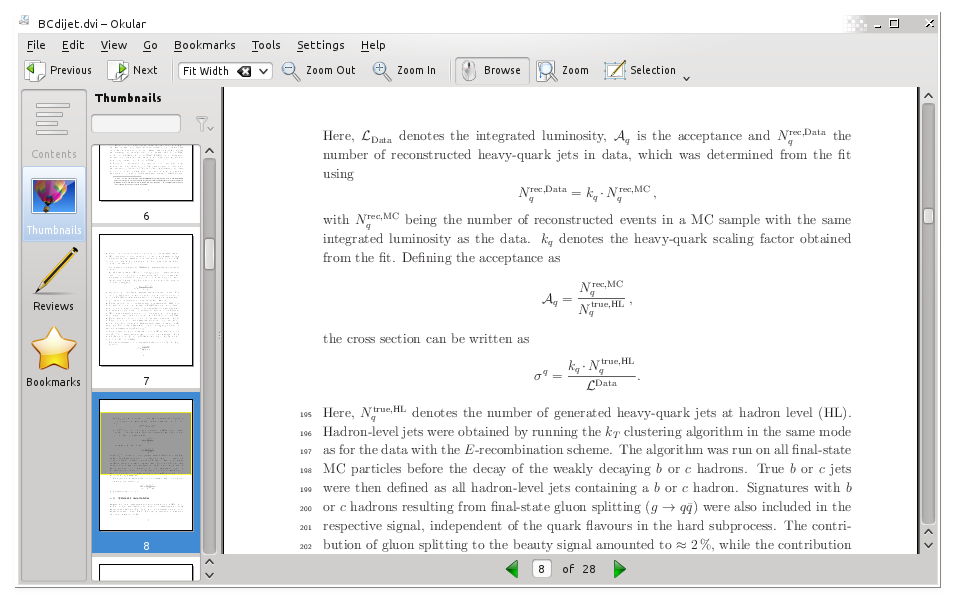
\includegraphics[width=7cm]{BCDijet} &
  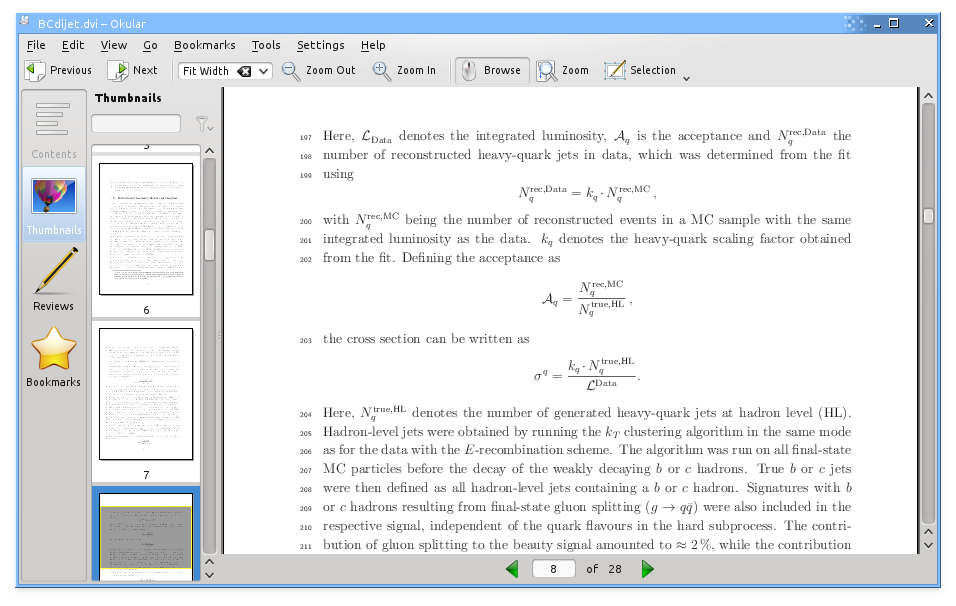
\includegraphics[width=7cm]{BCDijet-linenomath}\\
  (a) & (b)
  \end{tabular}
  \caption{Example of (a) a problem with line numbers and (b) its solution.}%
  \label{fig:lineno}
\end{figure}

Such problems are associated with text that is close to math mode
environments. Some of the problems can be solved by using a new
version of the \Package{lineno} package.
However, this only works for \enquote{standard} \LaTeX{}
math environments: \Env{displaymath}, \Env{equation} and \Env{eqnarray}, while it does
not work for recommended \Package{amsmath} environments such as \Env{equation*},
\Env{align(*)} and \Env{alignat(*)}. % chktex 36

The solution is to enclose the equation in \Env{linenomath} environment, e.g.
\begin{tcblisting}{listing only}
The total visible cross section for inclusive heavy-quark jet
production, \(\sigma^{q}\), with \(q\in\{b,c\}\) is given by
\begin{linenomath}
\begin{equation*}
  \sigma^{q} = \frac{N_{q}^{\text{rec,Data}}}%
    {\mathcal{A}_{q}\cdot\mathcal{L}_{\text{Data}}}.
\end{equation*}
\end{linenomath}
Here, \(\mathcal{L}_{\text{Data}}=\) denotes the integrated luminosity,
\(\mathcal{A}_{q}\) is the acceptance and \(N_{q}^{\text{rec,Data}}\) the
number of reconstructed heavy-quark jets in data, which was determined
\end{tcblisting}
\noindent
Then the line numbering will be correct, see \cref{fig:lineno}b.

The ATLAS \Package{atlasdoc} class contains a patch that gets round this problem.


%------------------------------------------------------------------------------
\section{Updating \Package{ubonn-thesis}}%
\label{sec:tips:update}\index{updating}\index{ubonn-thesis!updating}
%------------------------------------------------------------------------------

When you make a new thesis skeleton (as of version 2.1) the files
\texttt{thesis\_skel/Makefile} and \texttt{ubonn-thesis.sty}
(and \texttt{ubonn-biblatex.sty}) are copied
to your \texttt{mythesis} directory.
As of version 6.0, your \File{mythesis} directory should be completely standalone
and does not rely on any files in the parent directory.
If you want to profit from updates to \Package{ubonn-thesis},
you therefore need to copy the new version into \texttt{mythesis} again.
The advantage of this scheme is
that you can easily check what the differences are before you do the
copy. More importantly, if you have made your own changes to the style
file, it should be relatively easy to merge the two versions. Having
all files in the \texttt{mythesis} subdirectory also makes it much easier
for you to use your own version manager for your thesis.

What is therefore the best way to update \Package{ubonn-thesis}?
If you are using Git, then you first need to do a \Command{git pull}
in the \File{ubonn-thesis} directory.
If you use a tar file, then you should unpack it and copy over your
\texttt{mythesis} directory tree to the new \File{ubonn-thesis} tree.
As of version 6.0, you can then use a command like
\Command{make update THESIS=mythesis} to copy the style files,
the \File{Makefile}, the bib file with the standard references and the covers to your
\File{mythesis} directory.
You will be asked before existing files are overwritten.
If you overwrite the \File{Makefile} make sure you update the value of \Command{THESIS} afterwards.

As a side remark, I would also recommend that you put all Feynman
graphs etc.\ in subdirectories of \texttt{mythesis}. You may have to
change some variables that are set at the beginning of the
\texttt{Makefile} so that this works if you use \Package{feynmf}. If
you use \Package{feynmp} just add \Macro{write18} statements.
See \cref{sec:fig:feynman} for some more details.
